\chapter{General Introduction XXX}

\section{Trait-based ecology}
Understanding the structure and functioning of ecological communities is crucial if we are to unravel the effects of an ever-changing environment on terrestrial and marine ecosystems. In former times, ecologist relied on a species-based approach to explain the response of ecological communities and ecosystems to the variability of the environment. Since recently, investigating the variation of functional traits and their linkages to environmental gradients is emerging as a complementary, powerful approach \citep{McGill2006,Violle2007}. 

Traits are described as: "a well-defined, quantifiable properties of organisms, usually measured at the individual level and used comparatively across species" \citep{McGill2006}. If traits influence the fitness of organisms by affecting growth, reproduction, or survival, then they are called functional traits \citep{Violle2007}.  An organism may be characterized by several different traits, which tend to fall into three main categories: morphological, physiological, and behavioural traits. Under the scope of the energy allocation principle, the organisms divide the uptaked resources among different traits to maximize their fitness \citep{Perrin1993}. The cost of investing in one trait over the other is defined as a trade-off. Thus, a trade-off is a negative relationship between two traits where an increase in one is associated with a decrease in the other \citep{Tilman2000}.

A trait-based perspective in ecology promotes generality and predictability, thus closing the gap between developments in empirical and theoretical ecology. The focus of the trait-based modelling approach proposed in this thesis allows one to study ecological communities as single adaptive systems by focusing on macroscopic properties such as total biomass, mean trait value and trait variance. This leads to an understanding of processes such as species succession \citep{Bruggeman2009} or species variations and compositions \citep{Ackerly2007,Messier2010} in complex communities, processes that would otherwise be untreatable given the daunting high number of species typically comprising an ecological community or ecosystem.

The species-based approach is the classical perspective in which the role of each individual organism is considered in a community or ecosystem. In this approach, the studies of higher hierarchical ecological entities (i.e. populations, communities, ecosystems) are based on the understanding of the organism and species variations and on their responses to the changes in the environment. Many important processes are studied with this perspective, including competition, predation, and biodiversity \citep{Begon2006}. 

To compare the trait-based approach with the species-based approach, we can consider a simple thought experiment. Let us imagine a hypothetical phytoplankton community on a temperate region of the world, this community is composed of $n$ number of species and with a range of cell size from 0.2 to 200 $\mu$m. Different species with specific cell sizes will dominate the community at different times, depending on the environmental conditions. The community is subjected to temporal variations in light and nutrients, thus leading to continuous shifts in species composition (i.e. shifts in the dominant cell size). In this thought experiment, a species-based ecologist would study the shifts in species composition by considering the individual responses of the species to those temporal environmental changes. A trait-based ecologist, instead, would investigate the changes in the mean size values and size variance to the different environmental conditions. These features highlight the complementary of the two approaches, an aspect that has important implications when developing complex adaptive models for ecological systems.

\section{Phytoplankton trait-based community ecology}
Phytoplankton organisms are of global importance because of the key role they play in aquatic food webs and in the biogeochemical cycles of major nutrients (i.e. nitrogen, phosphorus and carbon). The study of phytoplankton community structure, also promoted by the work of \citet{Falkowski1998}, is therefore very relevant in marine ecology and is especially important for understanding how phytoplankton will respond to a changing climate and with which consequences.

Studies on the phytoplankton community composition and their response to the environmental gradients are not novel. Ramón Margalef was probably one of the first ecologist to give an important momentum to the topic.  \citep{Margalef1978} used observations of key traits, such as nutrient utilization and sinking rates, to support his well known concept called "Margalef's mandala". His classification of phytoplankton functional types (PFTs) at different nutrient and turbulent environmental conditions represents an excellent first example of how the trait-based notion can be applied to better understand phytoplankton community ecology, therefore setting up the stage for further developments in the field.

Phytoplankton can be characterised by many morphological, physiological, behavioural and life history traits and trade-offs \citep{Litchman2008, Litchman2010}. Key functional traits are generally associated with energy and resource allocation, edibility or predation avoidance, and reproductive strategies (Figure \ref{phytotrait}). However, among all the possibilities, the morphological trait $cell$ $size$ is the  most structuring property of phytoplankton communities \citep{Litchman2008, Finkel2009a, Litchman2010}, influencing many different ecological functions, processes and performances in these organisms. 

\subsection{Cell size as a major trait for characterising phytoplankton community structure}
The cell size has a major influence on many physiological and ecological processes, including growth, photosynthesis, nutrient acquisition, sinking rates, grazing, population abundance, and diversity \citep{Finkel2009a}. Phytoplankton cell size varies across a wide range, from picoplankton ($<$2 $\mu$m) to macroplankton (200 to $<$2000 $\mu$m). Many of the processes related to size can be described using a simple power law function: $Size \propto aV^ b$, where $V$ is the cell volume or biomass and $a$ and $b$ coefficients related to the specific species. This simple function has been proposed as a kind of universal law in biology \citep{Platt1981}. Phytoplankton growth and intracellular concentrations of nutrients and carbon, for example, have been found to be negatively related to cell size \citep{Tang1995}, suggesting that larger cells grow slower than smaller cells. 

\begin{figure}
\centering
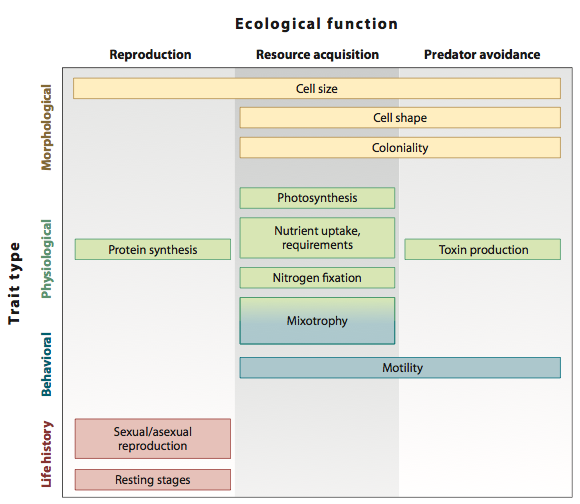
\includegraphics[width=0.7\linewidth]{./Chp1-Intro/Fig_litchman2008.png}
\caption[Scheme]{\small{Phytoplankton functional traits. Taken from \citet{Litchman2008}}}
\label{phytotrait}
\end{figure}

In a similar fashion one can determine the trade-off between size and metabolic processes. Results of studies focusing on this functional relation suggest that respiration rates increase with cell size \citep{Laws1975, Lopez-Urrutia2006} while photosynthetic rates, light absorption and pigment concentration decrease with cell size \citep{Ciotti2002,Finkel2004}. This evidence indicates that under light-limited conditions smaller cells are more efficient using the little energy available, probably due to a stronger package effect on larger cells. In this context the package effect is define as: "shading" effect of increased concentration of phytosynthetic pigments  which leads to a reduction in the light absorption efficiency \citep{Maranon2009}. However, this effect is "masked" under natural conditions due to the assemblage of many species comprising a community. Some species (especially larger ones) posses specific strategies that help them maintaining higher metabolic rates under adverse conditions \citep{Maranon2009}. 

Nutrient uptake decreases with decreasing cell size. But the advective transport of nutrients is enhanced by turbulence, sinking, and swimming, all aspects that increase the flux of nutrients from the cell diffusive boundary layer thus favouring larger cell organisms over smaller cell organisms \citep{Kiorboe1993}. However, small phytoplankton could also benefit from the smaller surface to area ratios, which provides them with a competitive advantage under low nutrient conditions.

Sinking velocity is also associated with size. This dynamics can be described by Stoke's law, predicting that sinking velocity increases with cell size \citep{Reynolds2006}. Larger organisms such as diatoms, however, can regulate buoyancy by changing their density \citep{Reynolds2006}. 

Other characteristics of higher hierarchical levels can also be described using an allometric relationship of size such as the population density, interspecific interactions and diversity. The abundance of certain population ($Num.cells/L$) can then be described as a function of input and output of nutrients, based on the Droop model \citep{Droop1977}, to scale up to species abundance \citep{Irwin2006}. Theoretical and empirical observations suggest that the popultaion abundance decreases with cell size \citep{Irwin2006,Cermeno2008}. 

Interspecific interactions, such as grazing, are also often size-specific. Larger grazers feed on larger phytoplankton with a predator to prey size ratio of 1:10 \citep{Kiorboe1993}. This interaction has the potential to regulate the trade-off between size-related nutrient uptake and predation avoidance \citep{Thingstad2005,Naselli-Flores2007}. 

The diversity of a community ($Num.species /L$) could be represented with a skewed log-normal distribution of the cell diameter, a mean cell diameter and a standard deviation on log scale \citep{Irwin2006}. In this functional relation, the highest diversity occurs at values smaller than the median \citep{Irwin2006, Cermeno2008a, Finkel2009a}. Although, phytoplankton are widely distributed they do not show any large-scale diversity pattern across latitudinal scales and productivity gradients. The involved mechanisms for such a lack of pattern could include: the high dispersal capabilities, the high patch connectivity, the chaotic biological interactions, the short generation times and the high frequency of environmental reset (e.i. the rapid change of species composition due to changes in the environment) \citep{Cermeno2008}. Thus, the governing process over phytoplankton diversity in large scales appears to be non-equilibrium dynamics as suggested by Hutchinson\citeyearpar {Hutchinson1961} in his plankton paradox tenet.

\section{Trait-based models of phytoplankton communities}
Early developments in plankton models were based on Lotka-Volterra predator-prey dynamics \citep{Fleming1939}. As advances in computational capabilities increased, models started to become more complex, up to a point where now the typical nutrient-phytoplankton-zooplankton-detritus (NPZD) models are resolved for various PFTs and then coupled to three-dimensional ocean circulation models. However, the increased number of PFTs in such models came with the cost of increased uncertainties, as reflected in increased number of  free parameters the models had to contain. The challenge today is thus to be able to develop models that incorporate all the essential organisms and the relevant processes, but on the same time that are manageable with a reasonable computing power and with as less degrees of freedom as possible. \citep{Anderson2010}.

In conclusion, the trait-based perspective, with its capability of describing a phytoplankton community as a single adaptive entity through just a few macroscopic properties (total biomass, mean trait, and trait variance), appears today to offer a simple and reliable framework which best suits modelling implementations. The species-based approach requires a more detailed knowledge of all the single species comprising an ecological community and leads to models with too many degrees of freedom. Even if computing and technical capabilities today may appear sufficient for several ecological applications, the complexity of natural interactions and the incredible number of organisms, each with specific strategic repertoires, would still set an important limit to the species-by-species modelling of phytoplankton communities.

Since trait-based modelling approaches are based on first principles, such as energy allocation theories \citep{Kooijman2009}, they lead to a mechanistic description of traits dynamics and, as mentioned above, to a reduce model complexity by considering the two most structuring traits subject to a well defined trade-off \citep{Merico2009, Follows2011}.

For phytoplankton communities, cell size appears to be the most suitable trait for this approach in particular when it is considered in relation to traits such as energy and nutrient allocation and susceptibility of being grazed (edibility) \citep{Litchman2008,Follows2011, Merico2009}. Trait-based models \citep{Bruggeman2007, Merico2009} have been so far quite successful at describing the community dynamics of phytoplankton. Some models specify a top-down control by including a detail representation of grazers. Advances in this field could include a trait-based definition of the zooplankton community, in analogy with the phytoplankton community. Further developments in modelling the phytoplankton community size-structure will help us to understand mechanisms that drive natural variation under changing environmental conditions.


\section{Aims of the proposed PhD project}
The general goal of my Ph.D. project is to study the processes that structure the phytoplankton community in contrasting environmental regions of the Atlantic Ocean, using a trait-based modelling perspective. The specific aims during the course of the project are to:

\begin{itemize}
\item Collect the appropriate dataset and available observations for developing a trait-based characterization of phytoplankton communities in contrasting regions of the Atlantic Ocean by using advanced statistical analyses. 
\item Implement a size-based model to understand the factors shaping the phytoplankton community structure in contrasting regions of the Atlantic and explore how communities re-organise under different environmental change scenarios.
\item Extend the proposed size-based model to incorporate a trait-based mechanistic description also for the zooplankton community and investigate the co-adaptation of these two different guilds under a changing environment.
\item If time allows, set up the model for long-term evolutionary studies in order to understand the factors that shapes phytoplankton size evolution through geological times.
\end{itemize}
